\documentclass[12pt,a4paper]{article}
\usepackage{lmodern}
\usepackage{amssymb,amsmath}
\usepackage{ifxetex,ifluatex}
\usepackage{fixltx2e} % provides \textsubscript
\ifnum 0\ifxetex 1\fi\ifluatex 1\fi=0 % if pdftex
  \usepackage[T1]{fontenc}
  \usepackage[utf8]{inputenc}
\else % if luatex or xelatex
  \ifxetex
    \usepackage{mathspec}
  \else
    \usepackage{fontspec}
  \fi
  \defaultfontfeatures{Ligatures=TeX,Scale=MatchLowercase}
    \setmainfont[]{Arial}
\fi
% use upquote if available, for straight quotes in verbatim environments
\IfFileExists{upquote.sty}{\usepackage{upquote}}{}
% use microtype if available
\IfFileExists{microtype.sty}{%
\usepackage{microtype}
\UseMicrotypeSet[protrusion]{basicmath} % disable protrusion for tt fonts
}{}
\usepackage[margin=1in]{geometry}
\usepackage{hyperref}
\hypersetup{unicode=true,
            pdftitle={Lista para Modelo Dinâmico},
            pdfauthor={Thiago Mendes Rosa},
            pdfborder={0 0 0},
            breaklinks=true}
\urlstyle{same}  % don't use monospace font for urls
\usepackage{color}
\usepackage{fancyvrb}
\newcommand{\VerbBar}{|}
\newcommand{\VERB}{\Verb[commandchars=\\\{\}]}
\DefineVerbatimEnvironment{Highlighting}{Verbatim}{commandchars=\\\{\}}
% Add ',fontsize=\small' for more characters per line
\usepackage{framed}
\definecolor{shadecolor}{RGB}{248,248,248}
\newenvironment{Shaded}{\begin{snugshade}}{\end{snugshade}}
\newcommand{\AlertTok}[1]{\textcolor[rgb]{0.94,0.16,0.16}{#1}}
\newcommand{\AnnotationTok}[1]{\textcolor[rgb]{0.56,0.35,0.01}{\textbf{\textit{#1}}}}
\newcommand{\AttributeTok}[1]{\textcolor[rgb]{0.77,0.63,0.00}{#1}}
\newcommand{\BaseNTok}[1]{\textcolor[rgb]{0.00,0.00,0.81}{#1}}
\newcommand{\BuiltInTok}[1]{#1}
\newcommand{\CharTok}[1]{\textcolor[rgb]{0.31,0.60,0.02}{#1}}
\newcommand{\CommentTok}[1]{\textcolor[rgb]{0.56,0.35,0.01}{\textit{#1}}}
\newcommand{\CommentVarTok}[1]{\textcolor[rgb]{0.56,0.35,0.01}{\textbf{\textit{#1}}}}
\newcommand{\ConstantTok}[1]{\textcolor[rgb]{0.00,0.00,0.00}{#1}}
\newcommand{\ControlFlowTok}[1]{\textcolor[rgb]{0.13,0.29,0.53}{\textbf{#1}}}
\newcommand{\DataTypeTok}[1]{\textcolor[rgb]{0.13,0.29,0.53}{#1}}
\newcommand{\DecValTok}[1]{\textcolor[rgb]{0.00,0.00,0.81}{#1}}
\newcommand{\DocumentationTok}[1]{\textcolor[rgb]{0.56,0.35,0.01}{\textbf{\textit{#1}}}}
\newcommand{\ErrorTok}[1]{\textcolor[rgb]{0.64,0.00,0.00}{\textbf{#1}}}
\newcommand{\ExtensionTok}[1]{#1}
\newcommand{\FloatTok}[1]{\textcolor[rgb]{0.00,0.00,0.81}{#1}}
\newcommand{\FunctionTok}[1]{\textcolor[rgb]{0.00,0.00,0.00}{#1}}
\newcommand{\ImportTok}[1]{#1}
\newcommand{\InformationTok}[1]{\textcolor[rgb]{0.56,0.35,0.01}{\textbf{\textit{#1}}}}
\newcommand{\KeywordTok}[1]{\textcolor[rgb]{0.13,0.29,0.53}{\textbf{#1}}}
\newcommand{\NormalTok}[1]{#1}
\newcommand{\OperatorTok}[1]{\textcolor[rgb]{0.81,0.36,0.00}{\textbf{#1}}}
\newcommand{\OtherTok}[1]{\textcolor[rgb]{0.56,0.35,0.01}{#1}}
\newcommand{\PreprocessorTok}[1]{\textcolor[rgb]{0.56,0.35,0.01}{\textit{#1}}}
\newcommand{\RegionMarkerTok}[1]{#1}
\newcommand{\SpecialCharTok}[1]{\textcolor[rgb]{0.00,0.00,0.00}{#1}}
\newcommand{\SpecialStringTok}[1]{\textcolor[rgb]{0.31,0.60,0.02}{#1}}
\newcommand{\StringTok}[1]{\textcolor[rgb]{0.31,0.60,0.02}{#1}}
\newcommand{\VariableTok}[1]{\textcolor[rgb]{0.00,0.00,0.00}{#1}}
\newcommand{\VerbatimStringTok}[1]{\textcolor[rgb]{0.31,0.60,0.02}{#1}}
\newcommand{\WarningTok}[1]{\textcolor[rgb]{0.56,0.35,0.01}{\textbf{\textit{#1}}}}
\usepackage{graphicx,grffile}
\makeatletter
\def\maxwidth{\ifdim\Gin@nat@width>\linewidth\linewidth\else\Gin@nat@width\fi}
\def\maxheight{\ifdim\Gin@nat@height>\textheight\textheight\else\Gin@nat@height\fi}
\makeatother
% Scale images if necessary, so that they will not overflow the page
% margins by default, and it is still possible to overwrite the defaults
% using explicit options in \includegraphics[width, height, ...]{}
\setkeys{Gin}{width=\maxwidth,height=\maxheight,keepaspectratio}
\IfFileExists{parskip.sty}{%
\usepackage{parskip}
}{% else
\setlength{\parindent}{0pt}
\setlength{\parskip}{6pt plus 2pt minus 1pt}
}
\setlength{\emergencystretch}{3em}  % prevent overfull lines
\providecommand{\tightlist}{%
  \setlength{\itemsep}{0pt}\setlength{\parskip}{0pt}}
\setcounter{secnumdepth}{5}
% Redefines (sub)paragraphs to behave more like sections
\ifx\paragraph\undefined\else
\let\oldparagraph\paragraph
\renewcommand{\paragraph}[1]{\oldparagraph{#1}\mbox{}}
\fi
\ifx\subparagraph\undefined\else
\let\oldsubparagraph\subparagraph
\renewcommand{\subparagraph}[1]{\oldsubparagraph{#1}\mbox{}}
\fi

%%% Use protect on footnotes to avoid problems with footnotes in titles
\let\rmarkdownfootnote\footnote%
\def\footnote{\protect\rmarkdownfootnote}

%%% Change title format to be more compact
\usepackage{titling}

% Create subtitle command for use in maketitle
\providecommand{\subtitle}[1]{
  \posttitle{
    \begin{center}\large#1\end{center}
    }
}

\setlength{\droptitle}{-2em}

  \title{Lista para Modelo Dinâmico}
    \pretitle{\vspace{\droptitle}\centering\huge}
  \posttitle{\par}
    \author{Thiago Mendes Rosa}
    \preauthor{\centering\large\emph}
  \postauthor{\par}
      \predate{\centering\large\emph}
  \postdate{\par}
    \date{20/06/2019}

\setlength\parindent{24pt}
\usepackage{indentfirst}
\usepackage[brazilian]{babel}
\usepackage[utf8]{inputenc}
\usepackage{indentfirst}
\usepackage{setspace}
\onehalfspace
\usepackage{color}
\usepackage{graphicx}
\usepackage{microtype}
\usepackage{enumitem}
\usepackage{amsmath}
\newtheorem{definition}{Definição}
\usepackage{pdfpages}
\usepackage{fancyhdr}
\usepackage{floatrow}
\usepackage{amsmath}
\usepackage{morefloats}
\usepackage{pbox}
\usepackage{graphicx}
\usepackage{xcolor, grffile}
\usepackage{color, colortbl}
\usepackage{tikz}
\usepackage{booktabs}
\usepackage{tabularx}
\floatplacement{figure}{H}
\floatsetup[figure]{capposition=top}
\floatsetup[table]{capposition=top}
\usepackage[bf]{caption}
\captionsetup{justification=raggedright,singlelinecheck=false}
\usepackage{placeins}
\usepackage{tocloft}
\usepackage{rotating}
\setlength{\cfttabnumwidth}{3em}
\setlength{\cftfignumwidth}{3em}

\begin{document}
\maketitle

\hypertarget{teoria}{%
\section{Teoria}\label{teoria}}

\hypertarget{modelo-economico}{%
\subsection{Modelo Econômico}\label{modelo-economico}}

Harold Zurcher gerencia uma frota de ônibus que é sujeita a todo tipo de
problema quando esta na rua. A milhagem (quilometragem) acumulada de um
ônibus \(x_t\) é a variável de estado do problema. O desgaste do ônibus
afeta o custo operacional esperado \(c(x_t; \theta_1)\) que depende da
milhagem e um vetor de parâmetros não conhecido
\(\theta_1 = \{\theta_{11}, . . . , \theta_{1n}\}\).

Assuma que os custos dos ônbius vem de dois componentes: manutenção
regular e despesas operacionais \(m(.)\) e o custo \(f(.)\) de
substituir o motor no caso de falha (que é um evento estocástico que
ocorre com alguma probabilidade).

\textbf{a) Escreva o custo como uma combinação destes dois componentes.
Indique claramente quais elementos são função de \(x_t\). Argumente
informalmente que \(\frac{\partial c}{\partial x_t} > 0\). Esta hipótese
é necessária para a solução do modelo. Ela é uma boa hipótese? Você pode
fazer um argumento para explicar por que
\(\frac{\partial c}{\partial x_t}\) poderia ser negativa (pelo menos
para alguns valores de \(x_t\))?}

\emph{Considere que o custo \(m(.)\) pode ser decomposto em
\(m(m_r(x_t),m_o(.))\), em que \(m_r\) denota as despesas com manutenção
regular e \(m_o\) as despesas operacionais. A função custo pode ser
escrita como \(c=(m(m_r(x_t),m_o(.)),f(x_t,.))\). Espera-se que, quanto
maior for a utilização de um ônibus da frota, maiores serão tanto os
custos de manutenção regular quanto os custos para substituição do motor
em caso de falha (numa eventual retifica do motor). Com isso, quanto
mais o ônibus roda, maior é o desgaste de suas peças e, portanto,
maiores serão os custos. O custo poderia diminuir com \(x_t\) em seus
valores iniciais se, por exemplo, houvesse uma garantia do fornecedor
para qualquer tipo de problema nas milhas iniciais ou pacotes de
manutenção até certo número de milhas inclusos com a compra do veículo.
\(\square\)}

\textbf{b) Rust não possui dados suficientes para estimar os vários
componentes da função custo, então ele simplesmente estimata
\(c(x_t, \theta_1)\). Que dados ele precisaria e que estratégia ele
poderia empregar se fosse querer identificar separadamente \(m()\) e
\(f()\)? Descreva qualquer hipótese que você precisa usar com os dados
para fazer funcionar a sua solução.}

\emph{Rust afirma que não estavam disponíveis dados detalhados de
manutenção e dos custos que envolvem a perda de clientes pela eventual
falha de funcionamento nos ônibus, um evento estocástico. Assim, não
seria possível decompor o custo como:}

\[
c(x,\theta_1) = m(x,\theta_{11}+\mu(x,\theta_{12})b(x,\theta_{13}))
\]

\emph{em que \((x,\theta_{11}\) é a esperança condicional das despesas
normais com manutenção e operação, \(\mu(x,\theta_{12})\) é a
probabilidade condicional de uma falha inesperada no motor e
\(b(x,\theta_{13})\) é a experança condicional dos custos relacionados a
troca do motor (reboque, troca de peças e perda de confiança do
consumidor). Assim, Rust estima apenas a soma desses componentes, \(c\).
Como a solução é especificar e estimar a soma dos custos, é preciso que
estes custos representem efetivamente separáveis em soma e não sejam
dependentes entre si. \(\square\)}

No começo de cada período \(t\) Harold Zurcher observa \(x_t\) e decide
quando pagar o custo de manutenção \(c(x_t, \theta_1)\) ou substituir o
motor, que instantaneamente leva a medida de uso para zero \(x_t = 0\).
Então, o benefício de um único período é dado por

\[ u(x_t,i_t,\theta) = 
  \begin{cases}
    -c(x_t,\theta)    & \quad \text{if } i_t=0\\
    R - c(0,\theta)  & \quad \text{if } i_t=1
  \end{cases}
\]

tal que \(R\) é o custo esperado de substituição do motor e \(i_t\) é a
decisão binária de investimento.

Faça \(F(x_{t+1}| x_t, i_t, \theta)\) representar a função de
distribuição cumulativa do processo estocástico que governa a evolução
da variável de estado.

\textbf{c) Escreva a equação de Bellman para este problema.}

\emph{Considere que o processo estocástico governando \(\{i_t,x_t\}\) é
solução para o seguinte problema de parada ótima regenerativo:}

\[
V_\theta(x_t)=\sup_\Pi \mathbb{E}\Bigg\{\sum_{j=t}^\infty \beta^{j-t}u(x_j,f_j,\theta_1)|x_t\Bigg\} 
\]

\emph{com a função utilidade definida anteriormente, \(\Pi\) sendo a
sequência infinita das regras de decisão \(\Pi=\{f_t,f_{t+1},...\}\),
\(f_t\) sendo a decisão de troca do motor no período \(t\), função de
toda a história do processo
\(i_t=f_t(x_t,i_{t-1},x_{t-1},i_{t-2},x_{t-2},...)\). A expectativa
anterior é tomada com respeito ao processo estocástico controlado
\(\{x_t\}\), cuja probabilidade é denotada por \(F\) (conforme definição
anter), cuja probabilidade de transição é:}

\[
F(x_{t+1}| x_t, i_t, \theta) = 
  \begin{cases}
    \theta_2exp\{\theta_2(x_{t+1}-x_t)\}    & \quad \text{if } i_t=0  \quad \text{and } x_{t+1} \geq x_t \\
    \theta_2exp\{\theta_2(x_{t+1})\}    & \quad \text{if } i_t=1  \quad \text{and } x_{t+1} \geq 0 \\
     0 &  \quad \text{otherwise}
  \end{cases}
\]

\emph{A equação acima tem a seguinte lógica: a milhagem acumulada advém
de uma distribuição exponencial quando o motor é mantido, considerando a
diferença entre o período futuro e o atual; Por outro lado, quando a
troca é efetuada, a milhagem se regenera e a distribuição exponencial da
milhagem acumulada é função apenas do período futuro.}

\emph{A função definida anteriormente, \(V_\theta(x_t)\), é o valor da
função, sendo solução única para a equação de Bellman, dada por:}

\[
V_\theta(x_t) = \max_{i_t \in C(x_t)}[u(x_t,i_t,\theta_1)+\beta\mathbb{E}V_\theta(x_t,i_t)]
\]

\emph{em que \(C(x_t)=\{0,1\}\) e \(\mathbb{E}V_\theta(x_t,i_t)\) é
definido como:}

\[
\mathbb{E}V_\theta(x_t,i_t)=\int_0^\infty V_\theta(y)p(dy|x_t,i_t,\theta_2) \quad \square
\]

Se pode obter uma solução analítica para a equação de Bellman em
\textbf{c)} assumindo que a distância percorrida em cada período é
distribuida exponencialmente com o parâmetro \(\theta_2\), que é
independente da milhagem rodada no período anterior: \[
F(x_{t+1} - x_t) = 1 - exp(-\theta_2(x_{t+1} - x_t))
\]

Fazendo isso implica em uma função política estacionária

\[ i(x_t,\theta) = 
  \begin{cases}
    1    & \quad \text{if } x_t \ge \gamma(\theta) \\
    0    & \quad \text{if } x_t < \gamma(\theta)
  \end{cases}
\]

tal que \gamma(\theta) é a solução única para

\[R(1-\beta) = \int_0^{\gamma(\theta)}[1 - \beta exp(-\theta_2(1 - \beta)y)]\frac{\partial c(y,\theta_1)}{\partial y}dy\]

Caso esteja interessado em detalhes deste modelo, ele foi derivado por
Rust em um paper anterior (``Stationary Equilibrium in a Market for
Durable Assets'', Econometrica 1985).

\textbf{d) Este modelo sofre de um problema de ``sobre-previsão''.
Explique o que significa. Se pode usar este modelo para estimação? Por
que ou por que não?}

\emph{Esta especificação implica em uma função de risco degenerada, na
qual, após certo limear, sempre é realizada a troca do motor
(\(x_t \ge \gamma(\theta)\)). Todavia, o autor aponta que os dados
refutam tal hipótese, uma vez que a troca do motor ocorre numa faixa de
milhagem muito ampla (de 82.400 a 387.000), sendo incompatível com uma
regra de limear a partir do qual a troca ocorre. Nesse sentido, ao
utilizar tal modelo, teríamos um ponto a partir do qual o motor do
ônibus é sempre trocado, algo não aderente a realidade. Assim sendo, a
utilização desse modelo para previsão não parece ser o mais adequado.
Como o autor aponta, a milhagem dos ônibus (\(x_t\)) não parece ser
apenas o único determinante para a troca do motor, existindo um conjunto
de outros fatores que podem influenciar tal decisão (o que levará a
adição do termo \(\varepsilon_t\) ao modelo). Além disso, assume-se que
\((x_{t+1}-x_t)\) tem uma distribuição exponencial i.i.d., fato refutado
pelo conjunto de dados analisado. \(\square\)}

\hypertarget{modelo-estocastico}{%
\subsection{Modelo Estocástico}\label{modelo-estocastico}}

Para estimar o comportamento que vemos nos dados é preciso adicionar
termos de erro ao modelo. Uma forma de fazer isso é assumindo que os
agentes desviam da solução ótima do modelo:

\[i_t = i(x_t, \theta) + \omega_t\]

Rust opta por uma estratégia diferente. Ele assume que os payoffs
recebem choques aleatórios \(\varepsilon_{it,t}\):

\[ U(x,i,\theta) = 
  \begin{cases}
    -c(x_t,\theta_1) + \varepsilon_{0,t}    & \quad \text{if } i_t=0\\
    R - c(0,\theta_1) + \varepsilon_{1,t}  & \quad \text{if } i_t=1
  \end{cases}
\]

\(\varepsilon_{it,t}\) é observado por Harold Zurcher, mas não pelo
econometrista.

\textbf{e) Interprete \(\omega_t\) e \(\varepsilon_t\). Que tipo de erro
eles representam? Discuta as vantagens e desvantagens de cada escolha de
modelagem. Por que você acha que Rust optou pela segunda opção?}

\emph{Em \(\omega_t\), tem-se um componente com variáveis de estado que
influenciam a decisão tomada pelo agente, mas desconhecida pelo
econometrista. O caso de \(\varepsilon_t\) é análogo, mas ele entra na
função utilidade, como sendo um componente da alternativa \(i\) no
período \(t\) que, igualmente, é conhecido pelo agente mas desconhecido
pelo econometrista. Rust argumenta que a primeira opção seria
internamente inconsistente, uma vez que o modelo estrutural partiu da
hipótese de que o comportamento do agente é compatível com a solução de
um problema de otimização dinâmico. A segunda abordagem trata o termo
estocástico de modo que ele seja internamente consistente, sendo
incorporado explicitamente na solução do problema, com a interpretação
de que \(\varepsilon_t\) é uma variável de estado não observável pelo
econometrista, mas pelo observada pelo agente. O autor comenta ainda que
essa estratégia garante um benefício adicional ao abrir a possibilidade
de que mais parâmetros possam ser estimados. \(\square\)}

\textbf{f) Escreva a nova função-valor \(V(x_t,\varepsilon_t)\)}

\[
V_\theta (x_t,\varepsilon_t) = \sup_\Pi \mathbb{E}\Bigg\{\sum_{j=t}^\infty \beta^{(j-t)}[u(x_j,f_j,\theta_1) + \varepsilon_j(f_j)]|x_t,\varepsilon_t,\theta_2,\theta_3 \Bigg\}
\]

\emph{Em que \(\Pi = \{f_t,f_{t+1},f_{t+2},...\}\),
\(f \in C(x_t), \forall t\), que é o conjunto de escolha, e a esperança
é tomada com respeito ao processo estocástico controlado
\(\{x_t,\varepsilon_t\}\) cuja densidade de probabilidade é definida a
partir de \(\Pi\) e a transição de probabilidade \(p\) é dada por:}

\[
dp\{x_{t+1},\varepsilon_{t+1},...,x_{N+1},\varepsilon_{N+1}|x_t,\varepsilon_t\} \\ = \prod_{i=t}^{N-1}p(x_{t+1},\varepsilon_{t+1}|x_{i},\varepsilon_{i},\theta_2,\theta_3) \quad \square
\]

Asolução para este problema é dada por uma regra de decisão estacionária
\(i_t = i(x_t,\varepsilon_t;\theta)\), que especifica a decisão ótima do
agente quando a variável de estado é \((x_t, \varepsilon_t)\). Neste
ponto, o modelo estatístico é completamente especificado mas ainda é
muito complicado de estimar -- especialmente com dados limitados.

\hypertarget{simplificando-as-hipoteses-para-estimacao}{%
\subsection{Simplificando as hipóteses para
estimação}\label{simplificando-as-hipoteses-para-estimacao}}

Rust fez as hipóteses simplificadoras
\(P (x_{t+1}; \varepsilon_{t+1}| x_t, \varepsilon_t) = P_1 ( x_{t+1}| x_t)P_2(\varepsilon_{t+1})\)
(ele chama isso de ``Conditional Independence Assumption'').

\textbf{g) Defina o valor esperado condicional de \(V(x_t)\) sobre
\(\varepsilon\) como}

\textbf{\[EV(x_t)= \int V(x_t;\varepsilon_t)P_2(\varepsilon_t)\]}

\textbf{Mostre que}

\[
\begin{aligned}
EV(x_t)=\mathbb{E}_t[\text{max}\{-c(x_t,\theta_1)+\varepsilon_{0,t} + \beta \int EV(x_{t+1})P(dx_{t+1}|x_t); \\ -R -c(0,\theta) + \varepsilon_{1,t} + \beta \int EV(x_{t+1})P(dx_{t+1}|0)\}]
\end{aligned}
\]

\emph{Ao assumir a ``Conditional Independence Assumption'' (CI), duas
restrições estão envolvidas. Conforme argumenta Rust, \(x_{t+1}\) é uma
estatística suficiente para \(\varepsilon_{t+1}\), o que significa que
\(x_{t+1}\) transmite qualquer dependência estatística entre
\(\varepsilon_{t}\) e \(\varepsilon_{t+1}\).}

\emph{Assim, aplicando o Teorema 1:}

\emph{Se}

\[G([u(x,\theta_1)+\beta EV_\theta(x)]|x,\theta_2) \\ \equiv \int_\varepsilon \max_{j \in C(x)} [u(x,j,\theta_1)+ \beta E V_\theta(x,j)]q(d\varepsilon|x,\theta_2)
\]

\emph{Então, \((P_i|x,\theta)\), dado por:}

\[
(P_i|x,\theta) = G_i([u(x,\theta_1)+ \beta EV_\theta(x)]|x,\theta_2)
\]

\emph{em que \(G_i\) denota a derivada parcial de \(G\) com respeito à
\(u(x,i,\theta_1)\) e a função \(EV_\theta\) é o único ponto fixo para
um mapeamento de contração \(T_\theta\),
\(T_\theta(EV_\theta)=EV_\theta\), definido para cada
\((x,i) \in \Gamma\) por:}

\[
EV_\theta(x,i)=\int_yG([u(y,\theta_1)+\beta EV_\theta (y)]|y,\theta_2)p(dy|x,i,\theta_3)
\]

\emph{Agora, basta passar a função de máximo para avaliar em qual estado
se tomara a esperança: em que a troca não é realizada
(\(-c(x_t,\theta_1)+\varepsilon_{0,t} + \beta \int EV(x_{t+1})P(dx_{t+1}|x_t)\))
ou em que ela é realizada
(\(-R -c(0,\theta) + \varepsilon_{1,t} + \beta \int EV(x_{t+1})P(dx_{t+1}|0)\))
\(\square\)}

\textbf{h) (*) Prove que a equação anterior é um mapeamento de contração
(contraction mapping).}

\emph{Primeiro, vamos colocar a definiição de contração:}

\begin{definition}
Seja $(X,d)$ um espaço métrico. Um mapeamento $T:X \rightarrow X$ é um mapeamento de contração, ou contração, se existe uma constante $c$, com $0 \leq c \leq 1$ tal que  

\[
d(T(x),T(y)) \leq cd(x,y)
\]

para todo $x,y \in X$

\end{definition}

\emph{Em palavras, uma contração mapeia pontos próximos. Como caso
particular, para todo ponto \(x \in X\), e qualquer \(r>0\), todos os
pontos na bola \(B_r(x)\) são mapeados para a bola \(B_s(Tx)\), com
\(r > s\). Se \(c < 1\), a contração pode ser chamada de estrita.}

\emph{Pela CI, temos um mapeamento do espaço
\(S=\{(x,\varepsilon\}|x \in R^k, \varepsilon \in R^\#C(x)\}\) para um
espaço contraído \(\Gamma=\{(x,i)|x \in R^k, i \in C(x)\}\). Sendo a
contraçaõ estrita, então existe um único ponto fixo, que, neste caso, é
o termo \(EV_\theta\) no espaço reduzido. \(\square\)}

\textbf{i) Explique o tradeoff resultante da hipótese de indenpendência
condicional (CI). Use um exemplo concreto para explicar o que é
descartado (ou deixado de lado). O que esta hipótese ``compra''
(i.e.~ela entrega) para a estimação? Essa hipótese é razoável?}

\emph{Ao adotar a CI, conforme apontado no item g), qualquer dependência
entre os termos não observados pelo econometrista depende apenas de
\(x_t\), o que acaba sendo uma hipótese forte, conforme Rust aponta.
Todavia, ao adotar tal estratégia, \(EV_\theta\) deixa de ser função do
termo não observado, dispensando que as pobrabilidades de escolham
envolvam uma integração sobre essa função desconhecida. Além disso, a CI
implica que \(EV_\theta\) é um ponto fixo de uma contração sobre o
espaço de estado reduzido (\(\Gamma=\{(x,i)|x\in R^k, i \in C(x)\}\) ao
invés de \(S=\{(x,i)|x\in R^k, \varepsilon \in R^{\#C(x)}\}\)), o que
confere mais um ganho computacional ao evitar o cômputo de mais uma
integral para obter \(EV_\theta\) a partir de \(V_\theta\). Ao fazer
isso, para o caso dos ônibus, as decisões de troca do motor não
observadas pelo econometristas em dois períodos podem depender de outras
coisas além da milhagem percorrida. O agente pode, por exemplo, observar
as condições das ruas ou a temperatura do ambiente (que pode afetar a
temperatura dos componentes do motor e acelerar seu desgaste) para
decidir sobre a troca do motor. Pode ainda, por exemplo, optar por
direcionar a troca do motor para o períodos em que a demanda por ônibus
é menor (como férias) de modo a diminuir eventuais impactos da troca do
motor. Todos esses fatores independem da milhagem \(x_t\), afetando a
escolha da troca. Apesar de ser uma hipótese forte, parece ser razoável
supor que \(x_t\) seja o principal fator a influenciar a parcela não
observada pelo econometrista}

Embora equação anterior seja uma contração, ainda é difícil computar sem
fazer hipóteses distribucionais adicionais sobre \(\varepsilon\). Rust
assume que o choque \(\varepsilon_{it,t}\)\$ segue uma distribuição
valor extremo Tipo I normalizada. Então:

\[
\varepsilon_{it,t} \sim EV1 \Bigg( \begin{bmatrix} 
0   \\ 0 \end{bmatrix}, \begin{matrix} \frac{\pi^2}{6} & 0 \\ 0 & \frac{\pi^2}{6} \end{matrix} \Bigg) 
\]

\textbf{j) Por que Rust escolheu uma distribuição padrão para o termo de
erro ao invés de adicionar um parâmetro para a sua variância?}

\emph{Conforme Rust aponta, um valor alto e negativo para
\(\varepsilon_t(0)\) pode ser interpretado como uma falha não observada
de algum componente do ônibus que força para a oficina, enquanto um
valor alto e positivo pode ser o reporte do motorista de que o ônibus
está bem ajustado. Já \(\varepsilon_t(1)\) pode ser associado ao custo
associado à troca do motor, em que um valor alto e negativo pode indicar
que não há espaço disponível para reparo ou que não existem motores
disponíveis para troca, enquanto um valor alto e positivo indica o
inverso. Como o autor não consegue identificar esses tipos de custo sem
informação adicional, ele optou por arbitrariamente normalizar a média e
variância.}

A hipótese de distribuição valor extremo nos permite derivar formas
funcionais para \(EV(x_t)\), e \(P(1 | x_t, \theta)\).

\textbf{k) Discuta a racionalidade por trás da hipótese da distribução
de \(\varepsilon_t\). Existem outras alternativas? Escolha uma
alternativa e discuta os prós e contras em relação à distribuição valor
extremo Tipo I.}

\emph{Ao escolher essa distribuição, o autor assume implicitamente que
\(\{x_t^j,\varepsilon_t^j\}\) são independentemente distribuídos entre
os diferentes ônibus, de menor relevância vis-à-vis sua hipótese de CI.
Uma outra possibilidade seria utilizar uma distribuição normal, como no
caso de um probit, o que lhe permitiria acomodar possíveis correlações
entre o processo decisório envolvendo a troca de motores dos ônibus.
Entretanto, isso levaria a complicações na definição do modelo,
demandando maiores informações sobre os custos que envolvem o processo
decisório de troca do motor.}

A última simplificação que Rust faz é discretizar o espaço de xt divindo
a milhagem em 90 intervalos de 5000 milhas. Ele assume que o processo xt
por avançar com pelo menos dois incrementos no tempo, que essencialmente
reduz a distribuição de \((x_{t+1} - x_t\)) como uma multinomial com
parâmetros \(\theta_3 = \{\theta_{30}, \theta_{31}\}\).

\textbf{l) Escreva \(P (x_{t+1}| x_t, i_t, \theta)\).}

\[
P (x_{t+1}| x_t, i_t, \theta) =
\begin{cases}
  g(x_{t+1} - x_t,\theta) & \quad \text{if } i_t=0 \\
  g(x_{t+1} - 0,\theta) & \quad \text{if } i_t=1
\end{cases}
\]

Aqui já se está em posição de estimar o modelo. As únicas duas coisas
que não foram especificadas são \(\beta\) e a forma da função custo.
Aqui podemos colocar \(\beta = 0.9999\)\footnote{\(\beta\) e \(R\) são
  em geral altamente colineares e portanto de difícil distinção. Para um
  tratamento rigoroso desta questão veja a seção 3.5 do capítulo escrito
  por Rust no Handbook of Econometrics (1994). Outra referência útil é o
  paper de Magnac e Thesmar (Econometrica, 2002).}. Finalmente, se pode
assumir que a função custo é linear:

\[
c (x_t, \theta_1) = 0.001 \theta_1 x_t
\]

\textbf{m) Observe que não foi incluída uma constante nesta
especificação de função custo. O que aconteceria se isto fosse feito?
Poderiamos estimar uma constante separadamente? Discuta como isso
impacta o resultado final de sua estimativa.}

\emph{Segundo Rust, o nível absoluto de \(c\) não é identificado uma vez
que a subtração de uma constante da função utilidade não afeta as
probabulidades de escolha. Assim, o que autor busca estimar, ao menos, a
mudança nos custos operacionais como função da distância percorrida
pelos ônibus, cuja normalização \(c(0,\theta_1)\) é utilizada}

\hypertarget{estimacao}{%
\section{Estimação}\label{estimacao}}

\hypertarget{dados}{%
\subsection{Dados}\label{dados}}

Primeiro é necessário construir a base de dados. A base consiste em oito
arquivos ASCII, contendo dados da leitura mensal do odômetro dos 162
ônibus do frota (Madison Metropolitan Bus Company). Estes dados são da
operação dos ônibus entre Dezembro de 1974 e Maio de 1985. Cada arquivo
corresponde a um modelo/categoria de ônibus da frota da Madison Metro:

\begin{enumerate}
\def\labelenumi{\arabic{enumi}.}
\tightlist
\item
  g870.ASC 36x15 matriz do modelo Grumman 870
\item
  rt50.ASC 60x4 matriz do modelo Chance RT50
\item
  t8h203.ASC 81x48 matriz do GMC T8H203
\item
  a452372.ASC 137x18 matriz do GMC A4523, modelo ano 1972
\item
  a452374.ASC 137x10 matriz do GMC A4523, modelo ano 1974
\item
  a530872.ASC 137x18 matriz do GMC A5308, modelo ano 1972
\item
  a530874.ASC 137x12 matriz do GMC A5308, modelo ano 1974
\item
  a530875.ASC 128x37 matriz do GMC A5308, modelo ano 1975
\end{enumerate}

Os dados em cada arquivo estão vetorizados em uma única coluna:
e.g.~g870.ASC é um vetor 540x1 consistindo nas colunas de uma matriz
110x4 que foi empilhada. Comece importando os dados e reorganizando cada
vetor em uma matriz. As primeiras 11 ``linhas'' de cada matriz consiste
no metadado:

\begin{Shaded}
\begin{Highlighting}[]
\CommentTok{#  Extrair tabela do PDF com a descrição das variáveis}

\NormalTok{tabulizer}\OperatorTok{::}\KeywordTok{extract_tables}\NormalTok{(}\StringTok{"lista2019.pdf"}\NormalTok{,}
                          \DataTypeTok{output =} \StringTok{"data.frame"}\NormalTok{)[[}\DecValTok{1}\NormalTok{]] }\OperatorTok
\StringTok{  }\NormalTok{dplyr}\OperatorTok{::}\KeywordTok{bind_rows}\NormalTok{(dplyr}\OperatorTok{::}\KeywordTok{bind_cols}\NormalTok{(}\DataTypeTok{Row=}\DecValTok{12}\NormalTok{, }
                                    \DataTypeTok{Field=}\StringTok{"Monthly odometer reading"}\NormalTok{,}
                                    \DataTypeTok{Sample.Entry=}\DecValTok{4235}\NormalTok{)) }\OperatorTok
\StringTok{  }\NormalTok{xtable}\OperatorTok{::}\KeywordTok{xtable}\NormalTok{(}\DataTypeTok{digits =} \KeywordTok{c}\NormalTok{(}\DecValTok{0}\NormalTok{,}\DecValTok{0}\NormalTok{,}\DecValTok{0}\NormalTok{,}\DecValTok{0}\NormalTok{),}
                 \DataTypeTok{caption=}\StringTok{"Dicionário de variáveis"}\NormalTok{) }\OperatorTok
\StringTok{  }\KeywordTok{print}\NormalTok{(}\DataTypeTok{include.rownames=}\NormalTok{F,}
                \DataTypeTok{comment=}\OtherTok{FALSE}\NormalTok{)}
\end{Highlighting}
\end{Shaded}

\begin{table}[ht]
\centering
\begin{tabular}{rlr}
  \hline
Row & Field & Sample.Entry \\ 
  \hline
1 & Bus ID & 5297 \\ 
  2 & Month purchased & 8 \\ 
  3 & Year purchased & 75 \\ 
  4 & Month of 1st engine replacement & 4 \\ 
  5 & Year of 1st engine replacement & 79 \\ 
  6 & Odometer reading at 1st engine replacement & 153400 \\ 
  7 & Month of 2nd engine replacement & 0 \\ 
  8 & Year of 2nd engine replacement & 0 \\ 
  9 & Odometer reading at 2nd engine replacement & 0 \\ 
  10 & Month odometer data begins & 9 \\ 
  11 & Year odometer data begins & 75 \\ 
  12 & Monthly odometer reading & 4235 \\ 
   \hline
\end{tabular}
\caption{Dicionário de variáveis} 
\end{table}

Você deve organizar os dados em objetos que são fáceis de manipular para
realizar a sua estimação. Em particular, observe que os dados do
odômetro NÃO são zerados quando o motor é substituído. Você deve
realizar esse ajuste. Importante: Todos os dados estão nos arquivos em
anexo, mas Rust roda o principal procedimento para um conjunto restrito
de ônibus. Esta restrição é devido a aparente heterogeneidade na matriz
de transição do espaço de estado entre os ônibus. Os arquivos que devem
ser usados para comparar com os resultados de Rust são 1, 2, 3 e 8.

Você deve organizar os dados em objetos que são fáceis de manipular para
realizar a sua estimação. Em particular, \emph{observe que os dados do
odômetro NÃO são zerados quando o motor é substituído. Você deve
realizar esse ajuste.}

\textbf{Importante:} Todos os dados estão nos arquivos em anexo, mas
Rust roda o principal procedimento para um conjunto restrito de ônibus.
Esta restrição é devido a aparente heterogeneidade na matriz de
transição do espaço de estado entre os ônibus. Os arquivos que devem ser
usados para comparar com os resultados de Rust são 1, 2, 3 e 8.

\begin{Shaded}
\begin{Highlighting}[]
\CommentTok{# Carregar a base de dados}

\CommentTok{#### Ler o dicionário de variáveis}
\CommentTok{#  Extrair tabela do PDF com a descrição das variáveis}
\NormalTok{dic <-}\StringTok{ }\NormalTok{tabulizer}\OperatorTok{::}\KeywordTok{extract_tables}\NormalTok{(}\StringTok{"lista2019.pdf"}\NormalTok{,}
                                 \DataTypeTok{output =} \StringTok{"data.frame"}\NormalTok{)[[}\DecValTok{1}\NormalTok{]]}

\CommentTok{# Listar arquivos com as bases de dados}
\NormalTok{bases<-}\StringTok{ }\KeywordTok{data.frame}\NormalTok{(}\DataTypeTok{arquivo=}\KeywordTok{list.files}\NormalTok{(}\StringTok{"rust_data"}\NormalTok{),}
                   \DataTypeTok{nome=}\KeywordTok{gsub}\NormalTok{(}\StringTok{".asc"}\NormalTok{,}\StringTok{""}\NormalTok{, }\KeywordTok{list.files}\NormalTok{(}\StringTok{"rust_data"}\NormalTok{)),}
                   \DataTypeTok{linhas=}\KeywordTok{c}\NormalTok{(}\KeywordTok{rep}\NormalTok{(}\DecValTok{137}\NormalTok{,}\DecValTok{4}\NormalTok{),}\DecValTok{128}\NormalTok{,}\DecValTok{36}\NormalTok{,}\DecValTok{60}\NormalTok{,}\DecValTok{81}\NormalTok{),}
                   \DataTypeTok{stringsAsFactors =}\NormalTok{ F)}

\CommentTok{# Looping para carregar as bases}
\ControlFlowTok{for}\NormalTok{(b }\ControlFlowTok{in}\NormalTok{ bases}\OperatorTok{$}\NormalTok{arquivo)\{}

  \CommentTok{# Ler a base de dados}
\NormalTok{  base <-}\StringTok{ }\NormalTok{data.table}\OperatorTok{::}\KeywordTok{fread}\NormalTok{(}\KeywordTok{paste0}\NormalTok{(}\StringTok{"rust_data/"}\NormalTok{,b))}
  
  \CommentTok{# Definir o número de linhas da matriz}
\NormalTok{  nl<-bases[bases}\OperatorTok{$}\NormalTok{arquivo}\OperatorTok{==}\NormalTok{b,]}\OperatorTok{$}\NormalTok{linhas}
  
  \CommentTok{# Definir número de meses existentes na base}
\NormalTok{  nm<-nl}\DecValTok{-12}\OperatorTok{+}\DecValTok{1}
  
  \CommentTok{# Criar objeto para receber os dados fixos de cada ônibus}
\NormalTok{  dados <-}\StringTok{ }\KeywordTok{c}\NormalTok{()}
  
  \CommentTok{# Criar um objeto para receber as informações mensais}
\NormalTok{  t<-}\KeywordTok{c}\NormalTok{()}

\CommentTok{# Criar um objeto para receber as referências}
\NormalTok{  ref<-}\KeywordTok{c}\NormalTok{()}

\CommentTok{# Iniciar looping para carregar as informações fixas,}
\CommentTok{# repetindo para o número de meses}
\ControlFlowTok{for}\NormalTok{(i }\ControlFlowTok{in} \DecValTok{1}\OperatorTok{:}\DecValTok{11}\NormalTok{)\{}
  
  \CommentTok{# Capturar as informações de cada ônibus}
  \KeywordTok{assign}\NormalTok{(}\KeywordTok{paste0}\NormalTok{(}\StringTok{"V"}\NormalTok{,i), }\KeywordTok{unlist}\NormalTok{(}\KeywordTok{rep}\NormalTok{(base[}\KeywordTok{seq}\NormalTok{(i,}\KeywordTok{nrow}\NormalTok{(base),nl),],nm)))}
  
  \CommentTok{# Juntar resultados}
\NormalTok{  dados <-}\StringTok{ }\KeywordTok{cbind}\NormalTok{(dados,}\KeywordTok{get}\NormalTok{(}\KeywordTok{paste0}\NormalTok{(}\StringTok{"V"}\NormalTok{,i)))}
  
\NormalTok{\}}

\CommentTok{# Retirar as informações mensais (odômetros)}
  
  \ControlFlowTok{for}\NormalTok{(j }\ControlFlowTok{in} \DecValTok{12}\OperatorTok{:}\NormalTok{nl)\{}
    
    
    \CommentTok{# Retirar para cada ônibus}
\NormalTok{    V12 <-}\StringTok{ }\NormalTok{base[}\KeywordTok{seq}\NormalTok{(j,}\KeywordTok{nrow}\NormalTok{(base),nl)]}
    
    \CommentTok{# Juntar resultados}
\NormalTok{    t <-}\StringTok{ }\KeywordTok{rbind}\NormalTok{(t,V12)}
\NormalTok{\}}

\CommentTok{# Criar um objeto com a referência,}
\CommentTok{# tendo como base o mês e ano inicial do odômetro}

  
  \ControlFlowTok{for}\NormalTok{(i }\ControlFlowTok{in} \KeywordTok{seq}\NormalTok{(}\DecValTok{10}\NormalTok{,}\KeywordTok{nrow}\NormalTok{(base),nl))\{}
    
    \CommentTok{# Capturar o mês inicial, o ano inicial, definir sempre o primeiro}
    \CommentTok{# dia de cada mês para transformar em data e criar a sequência de }
    \CommentTok{# meses conforme o número de meses(nm) disponíveis na base}
    
\NormalTok{    r <-}\StringTok{ }\KeywordTok{data.frame}\NormalTok{(}\DataTypeTok{ref=}\KeywordTok{seq}\NormalTok{(}
      \CommentTok{# Define a data}
\NormalTok{      lubridate}\OperatorTok{::}\KeywordTok{dmy}\NormalTok{(}\KeywordTok{paste}\NormalTok{(}\StringTok{"01"}\NormalTok{,base[i],}
\NormalTok{                           base[i}\OperatorTok{+}\DecValTok{1}\NormalTok{],}\DataTypeTok{sep =} \StringTok{"/"}\NormalTok{)),}
      \CommentTok{# Sequência mensal}
      \DataTypeTok{by=}\StringTok{"month"}\NormalTok{,}
      \CommentTok{# Pelo número de meses}
      \DataTypeTok{length.out =}\NormalTok{ nm))}
  
    \CommentTok{# Juntar resultados}
\NormalTok{    ref<-}\StringTok{ }\KeywordTok{rbind}\NormalTok{(ref,r)}
  
\NormalTok{\}}

\CommentTok{# Juntar a base final}
\KeywordTok{assign}\NormalTok{(bases[bases}\OperatorTok{$}\NormalTok{arquivo}\OperatorTok{==}\NormalTok{b,]}\OperatorTok{$}\NormalTok{nome,}
\KeywordTok{cbind}\NormalTok{(dados,}\DataTypeTok{V12=}\NormalTok{t) }\OperatorTok
\StringTok{  }\CommentTok{# Organizar por ônibus}
\StringTok{  }\NormalTok{dplyr}\OperatorTok{::}\KeywordTok{arrange}\NormalTok{(V1) }\OperatorTok
\StringTok{  }\CommentTok{# Trazer referência}
\StringTok{  }\NormalTok{dplyr}\OperatorTok{::}\KeywordTok{bind_cols}\NormalTok{(ref) }\OperatorTok
\StringTok{  }\CommentTok{# Ajustar odômetros para ocasião da troca}
\StringTok{  }\NormalTok{dplyr}\OperatorTok{::}\KeywordTok{mutate}\NormalTok{(}\DataTypeTok{V12_adj=}\KeywordTok{case_when}\NormalTok{(V12.V1}\OperatorTok{>}\NormalTok{V6}\OperatorTok{&}\NormalTok{V6}\OperatorTok{>}\DecValTok{0}\OperatorTok{~}\NormalTok{V12.V1}\OperatorTok{-}\NormalTok{V6,}
                                \OtherTok{TRUE}\OperatorTok{~}\NormalTok{V12.V1), }\CommentTok{# Primeira troca}
                \DataTypeTok{V12_adj=}\KeywordTok{case_when}\NormalTok{(V12.V1}\OperatorTok{>}\NormalTok{V9}\OperatorTok{&}\NormalTok{V9}\OperatorTok{>}\DecValTok{0}\OperatorTok{~}\NormalTok{V12.V1}\OperatorTok{-}\NormalTok{V9,}
                                \OtherTok{TRUE}\OperatorTok{~}\NormalTok{V12_adj), }\CommentTok{# Segunda troca}
                \DataTypeTok{troca=}\KeywordTok{ifelse}\NormalTok{(V12_adj}\OperatorTok{<}\KeywordTok{lag}\NormalTok{(V12_adj),}\DecValTok{1}\NormalTok{,}\DecValTok{0}\NormalTok{), }\CommentTok{# Criar indicador de troca}
                \DataTypeTok{troca=}\KeywordTok{ifelse}\NormalTok{(}\KeywordTok{is.na}\NormalTok{(troca)}\OperatorTok{==}\NormalTok{T,}\DecValTok{0}\NormalTok{,troca),}
                \DataTypeTok{estado=}\KeywordTok{cut}\NormalTok{(V12_adj,}
                           \DataTypeTok{breaks =} \KeywordTok{c}\NormalTok{(}\KeywordTok{seq}\NormalTok{(}\DecValTok{0}\NormalTok{,}\KeywordTok{max}\NormalTok{(V12_adj), }\DataTypeTok{by=}\DecValTok{5000}\NormalTok{),}\OtherTok{Inf}\NormalTok{),}
                           \DataTypeTok{labels =} \OtherTok{FALSE}\NormalTok{),}
                \DataTypeTok{difV12=}\NormalTok{V12_adj}\OperatorTok{-}\KeywordTok{lag}\NormalTok{(V12_adj),}
                \DataTypeTok{difV12=}\KeywordTok{ifelse}\NormalTok{(}\KeywordTok{is.na}\NormalTok{(difV12)}\OperatorTok{==}\NormalTok{T}\OperatorTok{|}\NormalTok{difV12}\OperatorTok{<}\DecValTok{0}\NormalTok{,V12_adj,difV12))) }\CommentTok{# Ajustar primeiro valor}

\CommentTok{# Remover objetos desnecessários}
\KeywordTok{rm}\NormalTok{(base,dados,r,ref,t,}\DataTypeTok{list=}\KeywordTok{ls}\NormalTok{(}\DataTypeTok{pattern =} \StringTok{"V}\CharTok{\textbackslash{}\textbackslash{}}\StringTok{d"}\NormalTok{),b,i,j,nl,nm)}
\NormalTok{\}}
\end{Highlighting}
\end{Shaded}

\hypertarget{computacao-i-nfxp-de-rust}{%
\subsection{Computação I: NFXP de
Rust}\label{computacao-i-nfxp-de-rust}}

Dada as observações
\((\{x_0, i_0\},\{x_1,i_1\} , . . . , \{x_T, i_T\})\) podemos escrever
uma função verossimilhança

\[
\ell (x_1,...,x_T,i_1,...,i_T|x_0,i_0,\theta) = \prod_{t=1}^T P(i_t|x_t,\theta).P(x_t|x_{t-1},i_{t-1},\theta)
\label{eq:2}
\]

Você deve ter fórmulas para \(P(i_t|x_t,\theta)\) e
\(P(x_t|x_{t-1},i_{t-1},\theta)\) da Parte 1 da lista.

Rust usa o seguinte procedimento:

\textbf{Passo 1:} Estime \(\hat{\theta_3}\) usando

\[
\ell^1 (x_1,...,x_T,i_1,...,i_T|x_0,i_0,\theta) = \prod_{t=1}^T P(x_t|x_{t-1},i_{t-1},\theta_3)
\]

\textbf{Passo 2}: Use as estimativas \(\hat{\theta_3}\) como valores
consistentes e a estimativa \((\hat{\theta_1},\hat{R})\) usando

\[
\ell^2 (x_1,...,x_T,i_1,...,i_T|\theta)= \prod_{t=1}^T P(i_t|x_t,\theta)
\]

Para implementar este método você precisará calcular \(EV(x_t)\) para
cada valor de \(\theta\) considerado o algoritmo de maxima
verossimilhança. Portanto, o seu código deve ser estruturado para ter um
algoritmo de ponto fixo ``interno'' que calcula \(EV(x_t)\) (usando a
expressão derivada na parte \textbf{k)} e um algoritmo de busca
``externo'' que maximiza a função de verossimilhança. Um bom ponto de
partida pode ser o \emph{payoff} do período ou mesmo o valor de
\(EV(x_t)\) computado na iteração anterior da estimação.

\textbf{Passo 3:} Usando \((\hat{\theta_1},\hat{R},\hat{\theta_3})\)
como um ponto inicial, use a função de verossimilhança completa para
obter uma estimativa eficiente dos parâmetros.

\textbf{n) Estime \((\theta_1, R,\theta_3)\) usando a metodologia de
Rust de maximização da função de verossimilhança na equação 2 (ou uma
função log-verossimilhança equivalente)}\footnote{Você pode cair em um
  problema de estimação porque sua linguagem de programação aproxima
  números bem pequenos para zero. Este é um problema quando estiver
  calculando (como você verá) \(log(exp(x_1) + exp(x_2))\) onde tanto
  \(x_1\) ou \(x_2\) (ou ambos) são números negativos bem grandes. Nesse
  caso, se sua linguagem de programação soluciona \(exp(x_1)= 0\), então
  \(log(exp(x_1) + exp(x_2))=x_2\), que é errado. Você pode encontrar
  uma descrição detalhada deste problema em
  \url{https://lips.cs.princeton.edu/computing-log-sum-exp/}. A solução
  consiste enssencialmente em tirar \(exp (x_1)\) da soma do log: \[
  log(exp(x_1) + exp(x_2))= log (exp(x_1).(1 + exp (x_2 - x_1))) \\
  = x_1 + log((1+exp(x_2-x_1)))
  \]}. \textbf{Você deve comparar os números que estimou com os obtidos
por Rust no seu paper (a tabela relevante é Table IX).}

\begin{Shaded}
\begin{Highlighting}[]
\KeywordTok{library}\NormalTok{(ggplot2)}
\KeywordTok{library}\NormalTok{(msm)}

\CommentTok{# Criar a base de dados com os grupos 1, 2 e 3}
\NormalTok{data=}\StringTok{ }\KeywordTok{rbind}\NormalTok{(g870[,}\KeywordTok{c}\NormalTok{(}\StringTok{"V1"}\NormalTok{,}\StringTok{"troca"}\NormalTok{,}\StringTok{"V12_adj"}\NormalTok{,}\StringTok{"estado"}\NormalTok{,}\StringTok{"difV12"}\NormalTok{)],}
\NormalTok{            rt50[,}\KeywordTok{c}\NormalTok{(}\StringTok{"V1"}\NormalTok{,}\StringTok{"troca"}\NormalTok{,}\StringTok{"V12_adj"}\NormalTok{,}\StringTok{"estado"}\NormalTok{,}\StringTok{"difV12"}\NormalTok{)],}
\NormalTok{            t8h203[,}\KeywordTok{c}\NormalTok{(}\StringTok{"V1"}\NormalTok{,}\StringTok{"troca"}\NormalTok{,}\StringTok{"V12_adj"}\NormalTok{,}\StringTok{"estado"}\NormalTok{,}\StringTok{"difV12"}\NormalTok{)])}

\CommentTok{# lower=min(data$difV12)}
\CommentTok{# upper=max(data$difV12)}
\CommentTok{# mu=mean(data$difV12)}
\CommentTok{# sigma=sd(data$difV12)}
\CommentTok{# }
\CommentTok{# p_x0 = msm::ptnorm(5000,mu,sigma,lower,upper)}
\CommentTok{# p_x1 = msm::ptnorm(10000,mu,sigma,lower,upper)-p_x0}
\CommentTok{# p_x2 = 1 - p_x1 - p_x0}
\CommentTok{# p = c(p_x0, p_x1, p_x2)}
\CommentTok{# }
\CommentTok{# p}

\CommentTok{# Verificar a probabilidade empírica da mudança em cada estado}
\NormalTok{p <-}\StringTok{ }\NormalTok{data }\OperatorTok
\StringTok{  }\NormalTok{dplyr}\OperatorTok{::}\KeywordTok{mutate}\NormalTok{(}\DataTypeTok{p=}\KeywordTok{cut}\NormalTok{(difV12,}
                      \DataTypeTok{breaks =} \KeywordTok{c}\NormalTok{(}\OperatorTok{-}\OtherTok{Inf}\NormalTok{,}\DecValTok{5000}\NormalTok{,}\DecValTok{10000}\NormalTok{,}\OtherTok{Inf}\NormalTok{),}
                      \DataTypeTok{labels =} \KeywordTok{c}\NormalTok{(}\StringTok{"p_x0"}\NormalTok{,}\StringTok{"p_x1"}\NormalTok{,}\StringTok{"p_x2"}\NormalTok{))) }\OperatorTok
\StringTok{  }\NormalTok{dplyr}\OperatorTok{::}\KeywordTok{group_by}\NormalTok{(p) }\OperatorTok
\StringTok{  }\NormalTok{dplyr}\OperatorTok{::}\KeywordTok{summarise}\NormalTok{(}\DataTypeTok{n=}\KeywordTok{n}\NormalTok{()) }\OperatorTok
\StringTok{  }\NormalTok{dplyr}\OperatorTok{::}\KeywordTok{ungroup}\NormalTok{() }\OperatorTok
\StringTok{  }\NormalTok{dplyr}\OperatorTok{::}\KeywordTok{mutate}\NormalTok{(}\DataTypeTok{n=}\NormalTok{n}\OperatorTok{/}\KeywordTok{sum}\NormalTok{(n))}

\NormalTok{p <-}\StringTok{ }\NormalTok{p}\OperatorTok{$}\NormalTok{n}

\CommentTok{# p_x0 é a chance de manutenção na mesma faixa de milhagem,}
\CommentTok{# p_x1 é a chance de passa para o status 2,}
\CommentTok{# enquanto p_x1 chance de estar no último status }

\CommentTok{# Decisão do agente}

\CommentTok{# Variável iniciais}
\CommentTok{# O custo de troca, os parâmetros de manutenção da função custo, }
\CommentTok{# e a taxa de desconto são definidas aqui.}
\CommentTok{# A taxa de desconto de beta = 0.9999}


\NormalTok{rc =}\StringTok{ }\DecValTok{20}
\NormalTok{theta1_}\DecValTok{1}\NormalTok{ =}\StringTok{ }\FloatTok{0.5}
\NormalTok{theta1_}\DecValTok{2}\NormalTok{ =}\StringTok{ }\FloatTok{0.01}
\NormalTok{beta =}\StringTok{ }\FloatTok{0.97}

\CommentTok{# Definição da função custo}

\NormalTok{custo_miope=}\ControlFlowTok{function}\NormalTok{(S, FCM, params, p)\{}
  
  \StringTok{"A função custo míope computa o custo esperado associado com}
\StringTok{  cada decisão para cada estado, }
\StringTok{  retornando um conjunto de decisões/estados de custo.}
\StringTok{    }
\StringTok{   Inputs:}
\StringTok{    * Um inteiro S, descrevendo os possíveis estados do ônibus}
\StringTok{    * A função de custo de manutenção FMC, que tem como input um vetor de parâmetros e estados}
\StringTok{    * O vetor params, como entrada para FMC. O primeiro elemento do vetor }
\StringTok{      é o custo de substituição cs.}
\StringTok{    * Um vetor (3x1) descrevendo os estados de transição de probabilidades }
\StringTok{        }
\StringTok{    Outputs:}
\StringTok{    * Uma matriz (Sx2) contendo os custos de manutenção e troca para os N }
\StringTok{      possíveis estados dos ônibus"}
  
\NormalTok{  cs =}\StringTok{ }\NormalTok{params[}\DecValTok{1}\NormalTok{]}
\NormalTok{  maint_cost =}\StringTok{ }\KeywordTok{rep}\NormalTok{(}\OtherTok{NA}\NormalTok{,S)}
\NormalTok{  repl_cost =}\StringTok{ }\KeywordTok{rep}\NormalTok{(}\OtherTok{NA}\NormalTok{,S)}
  
  \ControlFlowTok{for}\NormalTok{(s }\ControlFlowTok{in} \DecValTok{1}\OperatorTok{:}\NormalTok{S)\{}
\NormalTok{    maint_cost[s] =}\StringTok{ }\KeywordTok{FCM}\NormalTok{(s,params[}\OperatorTok{-}\DecValTok{1}\NormalTok{])}
\NormalTok{    repl_cost[s] =}\StringTok{ }\NormalTok{rc}
\NormalTok{  \}}
  
  \KeywordTok{cbind}\NormalTok{(maint_cost,repl_cost)}
\NormalTok{\}}

\CommentTok{# Possíveis formas para a função custo:}
\CommentTok{# Linear: FCM(s,theta)=theta_11*s}
\CommentTok{# Quadrática: FCM(s,theta)=theta_11*s+theta_12*s^2}
\CommentTok{# Exponencial: FCM(s,theta)=exp(theta_11*s)}
\CommentTok{# Log: FCM(s,theta)=log(theta_11+theta_12*s)}

\NormalTok{lin_cost=}\ControlFlowTok{function}\NormalTok{(s,params) s}\OperatorTok{*}\NormalTok{params[}\DecValTok{1}\NormalTok{]}
\NormalTok{quad_cost=}\ControlFlowTok{function}\NormalTok{(s,params) s}\OperatorTok{*}\NormalTok{params[}\DecValTok{1}\NormalTok{]}\OperatorTok{+}\NormalTok{s}\OperatorTok{^}\DecValTok{2}\OperatorTok{*}\NormalTok{params[}\DecValTok{2}\NormalTok{]}
\NormalTok{exp_cost=}\ControlFlowTok{function}\NormalTok{(s,params) }\KeywordTok{exp}\NormalTok{(s}\OperatorTok{*}\NormalTok{params[}\DecValTok{1}\NormalTok{])}
\NormalTok{log_cost=}\ControlFlowTok{function}\NormalTok{(s,params) }\KeywordTok{log}\NormalTok{(params[}\DecValTok{1}\NormalTok{] }\OperatorTok{+}\StringTok{ }\NormalTok{s}\OperatorTok{*}\NormalTok{params[}\DecValTok{2}\NormalTok{])}

\CommentTok{# Definição das escolhas de probabilidade, como função do vetor de custos}

\NormalTok{escolha_prob=}\ControlFlowTok{function}\NormalTok{(cost_array)\{}
  
  \CommentTok{# Retorna a probabilidade de cada escolha, }
  \CommentTok{# condicional a um vetor de custos.}
  
\NormalTok{  S =}\StringTok{ }\KeywordTok{nrow}\NormalTok{(cost_array)}
\NormalTok{  cost =}\StringTok{ }\NormalTok{cost_array}\OperatorTok{-}\KeywordTok{apply}\NormalTok{(cost_array,}\DecValTok{1}\NormalTok{,min) }\CommentTok{#toma a diferença pois 1) resultados são iguais}
                                            \CommentTok{# 2) mais estável com exp()}
\NormalTok{  util =}\StringTok{ }\KeywordTok{exp}\NormalTok{(}\OperatorTok{-}\NormalTok{cost)}
\NormalTok{  pescolha =}\StringTok{ }\NormalTok{util}\OperatorTok{/}\KeywordTok{rowSums}\NormalTok{(util)}
  
\NormalTok{  pescolha}
\NormalTok{\}}

\CommentTok{# Algoritmo do mapeamento de contração (gera a escolha de probabilidade "forward-looking")}

\NormalTok{contraction_mapping=}\ControlFlowTok{function}\NormalTok{(S, p, FCM, params, }\DataTypeTok{beta=}\NormalTok{beta, }\DataTypeTok{threshold=}\FloatTok{1e-9}\NormalTok{, }\DataTypeTok{suppr_output=}\OtherTok{FALSE}\NormalTok{)\{}
  
  \StringTok{"Computa o valor esperado não-míope do agente para cada decisão possível }
\StringTok{  e cada possível estado do ônibus.}
\StringTok{  A iteração é realizada até a diferença obtida entre o passo anterior e o atual}
\StringTok{  é menor que o limear.}
\StringTok{  Inputs:}
\StringTok{  * Um número finito de estados S}
\StringTok{  * Um vetor com as probabilidades de transição de estado p = [p(0), p(1), p(2), ..., p(k)] de tamanho k < S}
\StringTok{  * Uma função de manutenção de custos FMC}
\StringTok{  * Um vetor de parâmtros para a função custo}
\StringTok{  * Um fator de desconto beta (opcional)}
\StringTok{  * Um limear para convergência (opcional)}
\StringTok{  Outputs:}
\StringTok{  * A convergência para a escolha de probabilidade forward-looking e }
\StringTok{  míope para cada estado, condicional aos 'params'"}
  
\NormalTok{  achieved =}\StringTok{ }\OtherTok{TRUE}
  
  \CommentTok{# Inicialização das matrizes de estado de transição}
  \CommentTok{# ST_mat: descreve as probabilidades de transição de estado se os custos de manutenção ocorrem}
  \CommentTok{# RT_mat: Estado regenerado para 0 se o custo de troca acontece.}
  \CommentTok{# [a,b] = transição do estado "a" para "b"}
\NormalTok{  ST_mat =}\StringTok{ }\KeywordTok{matrix}\NormalTok{(}\DecValTok{0}\NormalTok{,S,S)}
\NormalTok{  lp =}\StringTok{ }\KeywordTok{length}\NormalTok{(p)}
  \ControlFlowTok{for}\NormalTok{(i }\ControlFlowTok{in} \DecValTok{1}\OperatorTok{:}\NormalTok{S)\{}
    \ControlFlowTok{for}\NormalTok{(j }\ControlFlowTok{in} \DecValTok{1}\OperatorTok{:}\NormalTok{lp)\{}
      \ControlFlowTok{if}\NormalTok{((i}\OperatorTok{+}\NormalTok{j}\DecValTok{-1}\NormalTok{)}\OperatorTok{<}\NormalTok{S)  ST_mat[i,i}\OperatorTok{+}\NormalTok{j}\DecValTok{-1}\NormalTok{] =}\StringTok{ }\NormalTok{p[j]}
      \ControlFlowTok{if}\NormalTok{((i}\OperatorTok{+}\NormalTok{j}\DecValTok{-1}\NormalTok{)}\OperatorTok{==}\NormalTok{S) ST_mat[i,i}\OperatorTok{+}\NormalTok{j}\DecValTok{-1}\NormalTok{] =}\StringTok{ }\KeywordTok{sum}\NormalTok{(p[j}\OperatorTok{:}\NormalTok{lp]) }\CommentTok{#sobre as colunass (probabilidades colapsadas)}
\NormalTok{    \}}
\NormalTok{  \}}
  
\NormalTok{  R_mat =}\StringTok{ }\KeywordTok{cbind}\NormalTok{(}\DecValTok{1}\NormalTok{,}\KeywordTok{matrix}\NormalTok{(}\DecValTok{0}\NormalTok{,S,S}\DecValTok{-1}\NormalTok{))}
  
  \CommentTok{# Inicialização do valor esperado (que também é a decisão de custo do agente míope).}
  \CommentTok{# Aqui, o componente forward-looking é inicializado em 0.}
\NormalTok{  k =}\StringTok{ }\DecValTok{0}
\NormalTok{  EV =}\StringTok{ }\KeywordTok{matrix}\NormalTok{(}\DecValTok{0}\NormalTok{,S,}\DecValTok{2}\NormalTok{)}
\NormalTok{  EV_miope =}\StringTok{ }\NormalTok{EV_nova =}\StringTok{ }\KeywordTok{custo_miope}\NormalTok{(S, FCM, params, p)}
  
  \CommentTok{# Contraction mapping loop}
  \ControlFlowTok{while}\NormalTok{(}\KeywordTok{max}\NormalTok{(}\KeywordTok{abs}\NormalTok{(EV_nova}\OperatorTok{-}\NormalTok{EV)) }\OperatorTok{>}\StringTok{ }\NormalTok{threshold)\{}
    \CommentTok{# Guardar o valor esperado anterior}
\NormalTok{    EV =}\StringTok{ }\NormalTok{EV_nova}
    \CommentTok{# Obter a probabilidade de manutenção e troca a partir do valor esperado anterior}
\NormalTok{    pescolha =}\StringTok{ }\KeywordTok{escolha_prob}\NormalTok{(EV)}
    \CommentTok{# Computar o custo esperado para cada estado: vetor Nx1}
\NormalTok{    ecost =}\StringTok{ }\KeywordTok{rowSums}\NormalTok{(pescolha}\OperatorTok{*}\NormalTok{EV)}
    \CommentTok{# Computar os dois componentes da utilidade forward-looking: }
    \CommentTok{# No caso de manutenção, a utilidade dos futuros estados ponderada pela}
    \CommentTok{# probabilidade de transição. No caso de troca,}
    \CommentTok{# a utilidade futura é a utilidade do estado 0}
\NormalTok{    futil_maint =}\StringTok{ }\NormalTok{ST_mat}\OperatorTok\NormalTok{ecost}
\NormalTok{    futil_repl =}\StringTok{ }\NormalTok{R_mat}\OperatorTok\NormalTok{ecost}
\NormalTok{    futil =}\StringTok{ }\KeywordTok{cbind}\NormalTok{(futil_maint,futil_repl)}
    \CommentTok{# A utilidade futura é descontada por beta, e adicionado ao custo míope. }
\NormalTok{    EV_nova =}\StringTok{ }\NormalTok{EV_miope }\OperatorTok{+}\StringTok{ }\NormalTok{beta}\OperatorTok{*}\NormalTok{futil}
\NormalTok{    k =}\StringTok{ }\NormalTok{k}\OperatorTok{+}\DecValTok{1}
    \ControlFlowTok{if}\NormalTok{(k }\OperatorTok{==}\StringTok{ }\DecValTok{1000}\NormalTok{) achieved =}\StringTok{ }\OtherTok{FALSE}
\NormalTok{  \}}
  
  \ControlFlowTok{if}\NormalTok{(}\OperatorTok{!}\NormalTok{suppr_output)\{}
    \ControlFlowTok{if}\NormalTok{(achieved)\{}
      \KeywordTok{cat}\NormalTok{(}\StringTok{"Convergence achieved in "}\NormalTok{,k,}\StringTok{" iterations"}\NormalTok{)}
\NormalTok{    \} }\ControlFlowTok{else}\NormalTok{ \{}
      \KeywordTok{cat}\NormalTok{(}\StringTok{"CM could not converge! Mean difference = "}\NormalTok{,}\KeywordTok{round}\NormalTok{(}\KeywordTok{mean}\NormalTok{(EV_nova}\OperatorTok{-}\NormalTok{EV),}\DecValTok{2}\NormalTok{))}
\NormalTok{    \}}
\NormalTok{  \}}
  
  \KeywordTok{list}\NormalTok{(}\DataTypeTok{CP_forward=}\KeywordTok{escolha_prob}\NormalTok{(EV_nova),}\DataTypeTok{CP_miope=}\KeywordTok{escolha_prob}\NormalTok{(EV_miope))}
\NormalTok{\}}

\CommentTok{# IV. Generation of simulated data (using a linear cost specification)}

\CommentTok{# 1) True coefficients}

\CommentTok{# Here, we use the same coefficients as the one described earlier:}

\CommentTok{# Cost and discount coefficients:}
\CommentTok{# rc=20}
\CommentTok{# theta11=0.5}
\CommentTok{# theta12=0.01}
\CommentTok{# beta=0.75}

\CommentTok{# State transition probabilities: (Mileage_t+1-Mileage_t)~NTrunc(6000,4000), such that:}
\CommentTok{# p_x0=0.36}
\CommentTok{# p_x1=0.48}
\CommentTok{# p_x2=0.16}

\CommentTok{# Finally, we assume that there are 70 discrete states for the bus' mileage }
\CommentTok{# (i.e. no bus has a mileage greater than 345,000 in the dataset).}

\CommentTok{# 2) Choice probabilities, as a function of the bus' state:}

\CommentTok{# Using the Contraction Mapping algorithm implemented earlier, we can obtain the }
\CommentTok{# probabibility of maintenance as a function of the bus' state for a forward-looking}
\CommentTok{# agent and a myopic agent.}

\NormalTok{params_lin =}\StringTok{ }\KeywordTok{c}\NormalTok{(rc,theta1_}\DecValTok{1}\NormalTok{)}
\NormalTok{p =}\StringTok{ }\NormalTok{p}
\NormalTok{S =}\StringTok{ }\KeywordTok{length}\NormalTok{(}\KeywordTok{table}\NormalTok{(data}\OperatorTok{$}\NormalTok{estado))}
\NormalTok{out =}\StringTok{ }\KeywordTok{contraction_mapping}\NormalTok{(}\DataTypeTok{S=}\NormalTok{S, }\DataTypeTok{p=}\NormalTok{p, }\DataTypeTok{FCM=}\NormalTok{lin_cost, }\DataTypeTok{params=}\NormalTok{params_lin, }\DataTypeTok{beta =}\NormalTok{ beta)}
\end{Highlighting}
\end{Shaded}

\begin{verbatim}
## Convergence achieved in  704  iterations
\end{verbatim}

\begin{Shaded}
\begin{Highlighting}[]
\NormalTok{lin_forward=out}\OperatorTok{$}\NormalTok{CP_forward}
\NormalTok{lin_miope=out}\OperatorTok{$}\NormalTok{CP_miope}
\NormalTok{pescolha =}\StringTok{ }\NormalTok{lin_forward[,}\DecValTok{1}\NormalTok{]}

\NormalTok{ggdat1 =}\StringTok{ }\KeywordTok{data.frame}\NormalTok{(}\DataTypeTok{Regra=}\KeywordTok{c}\NormalTok{(}\KeywordTok{rep}\NormalTok{(}\StringTok{"Forward-Looking"}\NormalTok{,}\KeywordTok{nrow}\NormalTok{(lin_forward)),}
                                   \KeywordTok{rep}\NormalTok{(}\StringTok{"Míope"}\NormalTok{,}\KeywordTok{nrow}\NormalTok{(lin_forward))),}
                    \DataTypeTok{pMaint=}\KeywordTok{c}\NormalTok{(lin_forward[,}\DecValTok{1}\NormalTok{],lin_miope[,}\DecValTok{1}\NormalTok{]),}
                    \DataTypeTok{State=}\KeywordTok{rep}\NormalTok{(}\DecValTok{1}\OperatorTok{:}\NormalTok{S,}\DataTypeTok{times=}\DecValTok{2}\NormalTok{))}

\KeywordTok{ggplot}\NormalTok{(ggdat1,}\KeywordTok{aes}\NormalTok{(}\DataTypeTok{y=}\NormalTok{pMaint,}\DataTypeTok{x=}\NormalTok{State,}\DataTypeTok{color=}\NormalTok{Regra))}\OperatorTok{+}
\StringTok{  }\KeywordTok{geom_line}\NormalTok{(}\DataTypeTok{lwd=}\DecValTok{1}\NormalTok{)}\OperatorTok{+}
\StringTok{  }\KeywordTok{theme_bw}\NormalTok{(}\DecValTok{12}\NormalTok{)}\OperatorTok{+}
\StringTok{  }\KeywordTok{scale_x_continuous}\NormalTok{(}\DataTypeTok{breaks =} \KeywordTok{seq}\NormalTok{(}\DecValTok{0}\NormalTok{,}\KeywordTok{length}\NormalTok{(}\KeywordTok{unique}\NormalTok{(data}\OperatorTok{$}\NormalTok{estado)),}\DataTypeTok{by=}\DecValTok{5}\NormalTok{))}\OperatorTok{+}
\StringTok{  }\KeywordTok{scale_y_continuous}\NormalTok{(}\DataTypeTok{labels =}\NormalTok{ scales}\OperatorTok{::}\NormalTok{percent)}\OperatorTok{+}
\StringTok{  }\KeywordTok{labs}\NormalTok{(}\DataTypeTok{x=}\StringTok{"Estado"}\NormalTok{,}
       \DataTypeTok{y=}\StringTok{"Prob."}\NormalTok{)}
\end{Highlighting}
\end{Shaded}

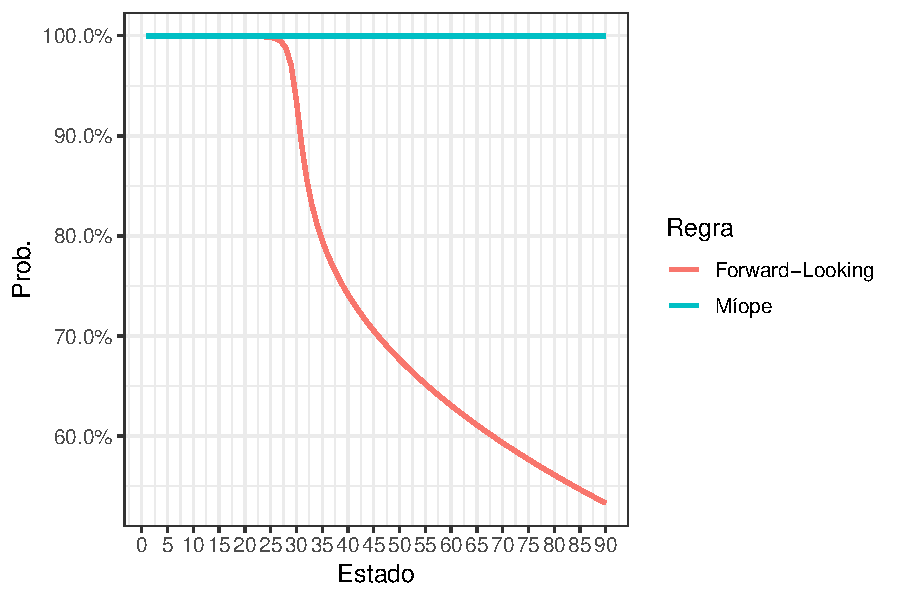
\includegraphics{Lista_econometria_II_files/figure-latex/unnamed-chunk-3-1.pdf}

\begin{Shaded}
\begin{Highlighting}[]
\CommentTok{# Estimação}

\CommentTok{# 1) Modelo Logit de utilidade dinâmica}


\CommentTok{# Grupo 1,2,3}
\NormalTok{data=}\StringTok{ }\KeywordTok{rbind}\NormalTok{(g870[,}\KeywordTok{c}\NormalTok{(}\StringTok{"V1"}\NormalTok{,}\StringTok{"troca"}\NormalTok{,}\StringTok{"V12_adj"}\NormalTok{,}\StringTok{"estado"}\NormalTok{)],}
\NormalTok{            rt50[,}\KeywordTok{c}\NormalTok{(}\StringTok{"V1"}\NormalTok{,}\StringTok{"troca"}\NormalTok{,}\StringTok{"V12_adj"}\NormalTok{,}\StringTok{"estado"}\NormalTok{)],}
\NormalTok{            t8h203[,}\KeywordTok{c}\NormalTok{(}\StringTok{"V1"}\NormalTok{,}\StringTok{"troca"}\NormalTok{,}\StringTok{"V12_adj"}\NormalTok{,}\StringTok{"estado"}\NormalTok{)])}

\CommentTok{# Grupo 4}
\CommentTok{# data2= rbind(a530875[,c("V1","troca","V12_adj","estado")])}

\CommentTok{# Grupo 1,2,3 e 4}
\CommentTok{# data3= rbind(g870[,c("V1","troca","V12_adj","estado")],}
\CommentTok{#             rt50[,c("V1","troca","V12_adj","estado")],}
\CommentTok{#             t8h203[,c("V1","troca","V12_adj","estado")],}
\CommentTok{#             a530875[,c("V1","troca","V12_adj","estado")])}

\NormalTok{dynamiclogit=}\ControlFlowTok{function}\NormalTok{(params,data,S,p,FCM)\{}
  
  \StringTok{"Avalia os parâmetros de custos subjacente ao padrão de troca do motor}
\StringTok{  do ônibus por um agente forward-looking.}
\StringTok{  }
\StringTok{  Inputs:}
\StringTok{  * Base de dados: um 'data.frame' com:}
\StringTok{    -escolha: nome da coluna contendo uma variável dummy de escolha endógena}
\StringTok{    -estado:nome da coluna contendo uma variável de estado exógeno }
\StringTok{  }
\StringTok{  * p: o vetor de transição de estado da variável exógena.}
\StringTok{      Exemplo: p = [0, 0.6, 0.4] significa que o ônibus irá  }
\StringTok{      mudar para o próximo estado de milhagem com probabilidade 0.6, }
\StringTok{      e para o segundo estado de milhagem 0.4.}
\StringTok{  }
\StringTok{  * FCM: Função de custo de manutenção, que deve deve ter como}
\StringTok{  primeiro argumento o estado s e como segundo argumento um vetor}
\StringTok{  de parâmetros."}
  
\NormalTok{  endog =}\StringTok{ }\NormalTok{data}\OperatorTok{$}\NormalTok{troca}
\NormalTok{  exog =}\StringTok{ }\NormalTok{data}\OperatorTok{$}\NormalTok{estado}
  
\NormalTok{  N=}\KeywordTok{length}\NormalTok{(endog)}
\NormalTok{  S=}\KeywordTok{max}\NormalTok{(exog)}\OperatorTok{*}\DecValTok{2} \CommentTok{# Assumes that the true maximum number states is twice the maximum observed state.}
  
  \CommentTok{# Matrices to speed up computations of the log-likelihood}
  
  \CommentTok{# A (SxN) matrix indicating the state of each observation}
\NormalTok{  state_mat=}\KeywordTok{matrix}\NormalTok{(}\DecValTok{0}\NormalTok{,S,N)}
  \ControlFlowTok{for}\NormalTok{(s }\ControlFlowTok{in} \DecValTok{0}\OperatorTok{:}\NormalTok{(S}\DecValTok{-1}\NormalTok{)) state_mat[s}\OperatorTok{+}\DecValTok{1}\NormalTok{,]=(exog}\OperatorTok{==}\NormalTok{s)}\OperatorTok{*}\DecValTok{1} \CommentTok{#Note 0 is a state, sum(state_mat)==N should be true}
  
  \CommentTok{# A (2xN) matrix indicating with a dummy the decision taken by the agent for each time/bus observation (replace or maintain)}
\NormalTok{  dec_mat =}\StringTok{ }\KeywordTok{rbind}\NormalTok{(}\KeywordTok{t}\NormalTok{(}\DecValTok{1}\OperatorTok{-}\NormalTok{endog),endog)}
  
  \StringTok{"}
\StringTok{  The log-likelihood of the Dynamic model is estimated in several steps.}
\StringTok{  1) The current parameters are supplied to the contraction mapping function}
\StringTok{  2) The function returns a matrix of decision probabilities for each state.}
\StringTok{  3) This matrix is used to compute the loglikelihood of the observations}
\StringTok{  4) The log-likelihood are then summed accross individuals, and returned}
\StringTok{  "}
  
\NormalTok{  util =}\StringTok{ }\KeywordTok{contraction_mapping}\NormalTok{(}\DataTypeTok{S=}\NormalTok{S, }\DataTypeTok{p=}\NormalTok{p, }\DataTypeTok{FCM=}\NormalTok{FCM, }\DataTypeTok{params=}\NormalTok{params, }\DataTypeTok{beta =}\NormalTok{ beta,}\DataTypeTok{suppr_output =} \OtherTok{TRUE}\NormalTok{)}
\NormalTok{  pescolha =}\StringTok{ }\NormalTok{util}\OperatorTok{$}\NormalTok{CP_forward}
\NormalTok{  logprob =}\StringTok{ }\KeywordTok{log}\NormalTok{(}\KeywordTok{t}\NormalTok{(state_mat)}\OperatorTok\NormalTok{pescolha)}
  \OperatorTok{-}\KeywordTok{sum}\NormalTok{(logprob}\OperatorTok{*}\KeywordTok{t}\NormalTok{(dec_mat))}
\NormalTok{\}}

\CommentTok{# 2) Fitting the linear cost data}

\CommentTok{# A. Fitting the true linear cost function to the data}

\CommentTok{# In this section, we fit the data generated by the linear cost function and recover the parameters RC and ??. We do it for different characterizations of the cost function, and thereby illustrate the consequences of a misspecification.}
\CommentTok{# Recall that in the linear model:}
\CommentTok{# RC=20}
\CommentTok{# theta11=0.5}

\NormalTok{bounds =}\StringTok{ }\KeywordTok{c}\NormalTok{(}\FloatTok{1e-9}\NormalTok{, }\OtherTok{Inf}\NormalTok{)}
\NormalTok{npars=}\DecValTok{2}
\NormalTok{lin_fit =}\StringTok{ }\KeywordTok{optim}\NormalTok{(}\DataTypeTok{par=}\KeywordTok{rep}\NormalTok{(.}\DecValTok{1}\NormalTok{,npars),}\DataTypeTok{fn=}\NormalTok{dynamiclogit,}\DataTypeTok{method=}\KeywordTok{c}\NormalTok{(}\StringTok{"L-BFGS-B"}\NormalTok{),}\DataTypeTok{lower=}\NormalTok{bounds[}\DecValTok{1}\NormalTok{],}\DataTypeTok{upper=}\NormalTok{bounds[}\DecValTok{2}\NormalTok{],}
                \DataTypeTok{data=}\NormalTok{data,}\DataTypeTok{S=}\NormalTok{S,}\DataTypeTok{p=}\NormalTok{p,}\DataTypeTok{FCM=}\NormalTok{lin_cost,}\DataTypeTok{control=}\KeywordTok{list}\NormalTok{(}\DataTypeTok{fnscale=}\DecValTok{1}\NormalTok{))}

\CommentTok{# Return the parameters obtained after fitting the likelihood function to the data.}
\NormalTok{loglike =}\StringTok{  }\NormalTok{lin_fit}\OperatorTok{$}\NormalTok{value}
\NormalTok{fit_params =}\StringTok{ }\NormalTok{lin_fit}\OperatorTok{$}\NormalTok{par}
\KeywordTok{cat}\NormalTok{(}\StringTok{"Log-Likelihood: "}\NormalTok{,loglike,}\DataTypeTok{fill=}\OtherTok{TRUE}\NormalTok{)}
\end{Highlighting}
\end{Shaded}

\begin{verbatim}
## Log-Likelihood:  1751.994
\end{verbatim}

\begin{Shaded}
\begin{Highlighting}[]
\KeywordTok{cat}\NormalTok{(}\StringTok{"RC: "}\NormalTok{,fit_params[}\DecValTok{1}\NormalTok{],}\DataTypeTok{fill=}\OtherTok{TRUE}\NormalTok{)}
\end{Highlighting}
\end{Shaded}

\begin{verbatim}
## RC:  0.1
\end{verbatim}

\begin{Shaded}
\begin{Highlighting}[]
\KeywordTok{cat}\NormalTok{(}\StringTok{"thetas: "}\NormalTok{,fit_params[}\OperatorTok{-}\DecValTok{1}\NormalTok{],}\DataTypeTok{fill=}\OtherTok{TRUE}\NormalTok{)}
\end{Highlighting}
\end{Shaded}

\begin{verbatim}
## thetas:  0.004619508
\end{verbatim}

\begin{Shaded}
\begin{Highlighting}[]
\CommentTok{#Compare with the true values}
\NormalTok{params_lin =}\StringTok{ }\KeywordTok{c}\NormalTok{(}\DecValTok{20}\NormalTok{,.}\DecValTok{5}\NormalTok{)}
\NormalTok{linEst =}\StringTok{ }\KeywordTok{contraction_mapping}\NormalTok{(}\DataTypeTok{S=}\NormalTok{S, }\DataTypeTok{p=}\NormalTok{p, }\DataTypeTok{FCM=}\NormalTok{lin_cost, }\DataTypeTok{params=}\NormalTok{fit_params, }\DataTypeTok{beta =}\NormalTok{beta)}
\end{Highlighting}
\end{Shaded}

\begin{verbatim}
## Convergence achieved in  637  iterations
\end{verbatim}

\begin{Shaded}
\begin{Highlighting}[]
\NormalTok{lin_forwardEst=linEst}\OperatorTok{$}\NormalTok{CP_forward}
\NormalTok{lin_myopicEst=linEst}\OperatorTok{$}\NormalTok{CP_miope}

\NormalTok{gglinEst =}\StringTok{ }\KeywordTok{data.frame}\NormalTok{(}\DataTypeTok{decisionRule=}\KeywordTok{c}\NormalTok{(}\KeywordTok{rep}\NormalTok{(}\StringTok{"Forward-Looking (Lin)"}\NormalTok{,}
                                         \KeywordTok{nrow}\NormalTok{(lin_forward)),}
                                     \KeywordTok{rep}\NormalTok{(}\StringTok{"Myopic (Lin)"}\NormalTok{,}\KeywordTok{nrow}\NormalTok{(lin_miope)),}
                                     \KeywordTok{rep}\NormalTok{(}\StringTok{"Forward-Looking (Lin Est.)"}\NormalTok{,}
                                         \KeywordTok{nrow}\NormalTok{(lin_forwardEst)),}
                                     \KeywordTok{rep}\NormalTok{(}\StringTok{"Myopic (Lin Est.)"}\NormalTok{,}
                                         \KeywordTok{nrow}\NormalTok{(lin_myopicEst))),}
                      \DataTypeTok{pMaint=}\KeywordTok{c}\NormalTok{(lin_forward[,}\DecValTok{1}\NormalTok{],}
\NormalTok{                               lin_miope[,}\DecValTok{1}\NormalTok{],}
\NormalTok{                               lin_forwardEst[,}\DecValTok{1}\NormalTok{],}
\NormalTok{                               lin_myopicEst[,}\DecValTok{1}\NormalTok{]),}
                      \DataTypeTok{State=}\KeywordTok{c}\NormalTok{(}\DecValTok{0}\OperatorTok{:}\NormalTok{(}\KeywordTok{nrow}\NormalTok{(lin_forward)}\OperatorTok{-}\DecValTok{1}\NormalTok{),}
                              \DecValTok{0}\OperatorTok{:}\NormalTok{(}\KeywordTok{nrow}\NormalTok{(lin_miope)}\OperatorTok{-}\DecValTok{1}\NormalTok{),}
                              \DecValTok{0}\OperatorTok{:}\NormalTok{(}\KeywordTok{nrow}\NormalTok{(lin_forwardEst)}\OperatorTok{-}\DecValTok{1}\NormalTok{),}
                              \DecValTok{0}\OperatorTok{:}\NormalTok{(}\KeywordTok{nrow}\NormalTok{(lin_myopicEst)}\OperatorTok{-}\DecValTok{1}\NormalTok{)))}

\KeywordTok{ggplot}\NormalTok{(gglinEst,}\KeywordTok{aes}\NormalTok{(}\DataTypeTok{y=}\NormalTok{pMaint,}\DataTypeTok{x=}\NormalTok{State,}\DataTypeTok{color=}\NormalTok{decisionRule))}\OperatorTok{+}
\StringTok{  }\KeywordTok{geom_line}\NormalTok{(}\DataTypeTok{lwd=}\DecValTok{1}\NormalTok{)}\OperatorTok{+}
\StringTok{  }\KeywordTok{theme_bw}\NormalTok{(}\DecValTok{12}\NormalTok{)}\OperatorTok{+}
\StringTok{  }\KeywordTok{scale_x_continuous}\NormalTok{(}\DataTypeTok{breaks =} \KeywordTok{seq}\NormalTok{(}\DecValTok{0}\NormalTok{,}\KeywordTok{length}\NormalTok{(}\KeywordTok{unique}\NormalTok{(data}\OperatorTok{$}\NormalTok{estado)),}\DataTypeTok{by=}\DecValTok{5}\NormalTok{))}\OperatorTok{+}
\StringTok{  }\KeywordTok{scale_y_continuous}\NormalTok{(}\DataTypeTok{labels =}\NormalTok{ scales}\OperatorTok{::}\NormalTok{percent)}
\end{Highlighting}
\end{Shaded}

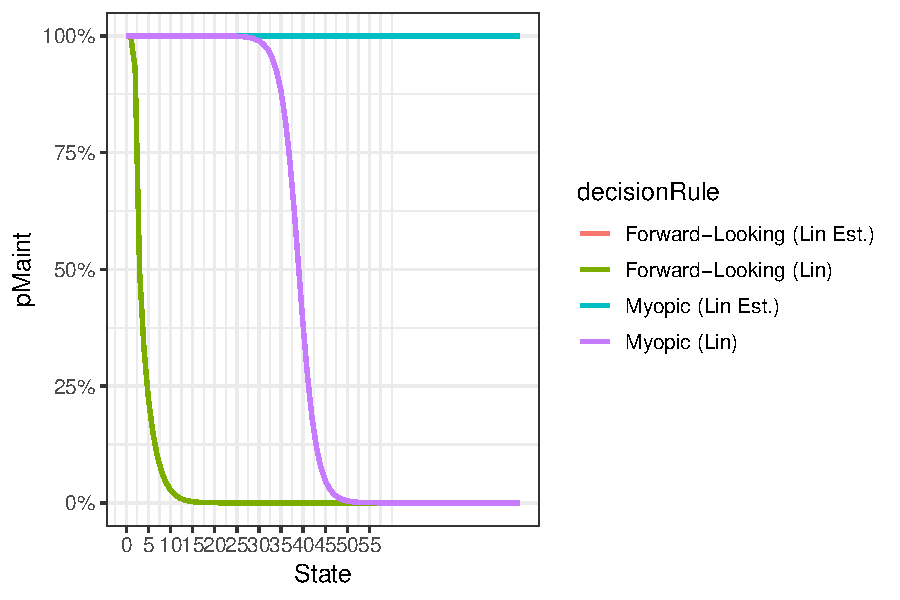
\includegraphics{Lista_econometria_II_files/figure-latex/unnamed-chunk-3-2.pdf}

\begin{Shaded}
\begin{Highlighting}[]
  \KeywordTok{labs}\NormalTok{(}\DataTypeTok{x=}\StringTok{"Estado"}\NormalTok{,}
       \DataTypeTok{y=}\StringTok{"Prob."}\NormalTok{)}
\end{Highlighting}
\end{Shaded}

\begin{verbatim}
## $x
## [1] "Estado"
## 
## $y
## [1] "Prob."
## 
## attr(,"class")
## [1] "labels"
\end{verbatim}

\textbf{o) Explique como você pode calcular os erros padrão para estes
coeficientes.}

\textbf{p) (*)) Calcule o erro padrão usando a metodologia que você
descreveu no item o).}

\textbf{q) (*) Rust estimou diferentes versões do seu modelo, variando
(i) a função custo, (ii) o parâmetro \(\beta\) e (iii) o número de
valores possíveis para a variável de estado \(x_t\). Ele relata alguns
resultados para todas parametrizações diferentes do modelo. Baseado
apenas no que ele apresenta no paper, argumente argumente quais destas
três hipóteses possuem maior consequência. Descreva e motive uma forma
de relaxar a hipótese (cabe a você desenvolver isto e fique a vontade
para usar uma das expansões apresentadas por Rust). Refaça a estimação
com esta hipótese relaxada. Comente sobre qualquer diferença relevante
nos resultados.}

\hypertarget{computacao-ii-metodo-ccp}{%
\subsection{Computação II: método CCP}\label{computacao-ii-metodo-ccp}}

O método de estimação montado por Rust é ``time-consuming'' porque
requer que você compute um ponto fixo para cada ``guess'' de \(\theta\).
Hotz e Miller propõem um método alternativo.

\textbf{r) Estime \(\hat{F}(x_{t+1}|x_t,i_t)\) a partir dos dados. Você
pode usar qualquer método (parametric, non-parametric, etc.). Justifique
sua escolha.}

\textbf{s) Estime \(\hat{P}(i_t=1|x_t)\) a partir dos dados. Novamente
justifique sua escolha de método.}

Agora faça

\[
\tilde{V} (i_t,x_t;\theta) \equiv \mathbb{E}_{\varepsilon_{i_{t},t}}[V(i_t,x_t,\varepsilon_t;\theta)]
\]

Uma vez que o termo de erro é média zero, temos

\[
\tilde{V} (i_t,x_t;\theta) \equiv -c(x_t,i_t;\theta_1) + \beta \mathbb{E}_{\varepsilon_{i_{t+1},t+1}}\Big[u(x_{t+1},i_{t+1};\theta)+\varepsilon_{i_{t+1},t+1}+\beta\mathbb{E}_{\varepsilon_{i_{t+2},t+2}}[\cdots]\Big]
\]

tal que as variáveis são distribuídas como

\[
x_{t+1} \sim \hat{F}(.|x_t,i_t) \\
i_{t+1} \sim \hat{P}(.|x_{t+1}) \\
x_{t+2} \sim \hat{F}(.|x_{t+1},i_{t+1}) \\
\]

e as expectativas são condicional, significando que elas são tomadas
mantendo a história fixa (e conhecida). As propriedades da distribuição
valor extremo Tipo I nos dizem que

\[
\mathbb{E}[\varepsilon_{i_{t},t}|i_t,x_t] = \gamma - log(P(i_t|x_t))
\]

tal que \(\gamma\) é a constante de Euler.

\textbf{t) Use um argumento recursivo para escrever
\(\tilde{V}(i_t,x_t;\theta)\) como uma soma infinitamente descontada
(infinite discounted sum).}

Você deve ser capaz de calcular a expressão que você derivou para
\(\tilde{V}(i_t,x_t;\theta)\) usando simulação numérica. Faça
\(\{(x_t^s,i_s^t)\}_{t=1,s=1}^{T,S}\) serem os valores simulados de
\(x_t\) e \(i_t\). Então você pode calcular
\(\tilde{V}^s(i_t^s,x_t^s;\theta)\) e obter uma estimativa consistente
de

\[
\tilde{V}^{sim}(i,x;\theta)=\frac{1}{S}\sum_{s=1}^S \tilde{V}^s(i_t^s,x_t^s;\theta)
\]

Seu \(\tilde{V}^{sim}\) deve ser uma função de q que é essencialmente
calculado para cada ``guess''. Observe que este passo deve fazer o
estimador mais rápido (uma vez que você não precisa computar a iteração
de ponto fixo toda vez que tiver um novo ``guess'' de \(\theta\).
Entretanto, o quão rápido será o seu estimador depende do quão
``objetivo'' (esperto) será a sua escolha de simulação. Em particular
tenha em mente o seguinte: (i) é mais rápido sortear um número de uma
matriz existente do que simular um número; e (ii) seus sorteios de
\((x_t^s , i_t^s )\) não dependem dos parâmetros que você está
estimando.

Para concluir o procedimento, relembre do começo que usando a hipótese
valor extremo T1

\[
\tilde{P}(i_t=1|x_t;\theta)=\frac{exp(\tilde{V}(x_t,i_t=1;\theta))}{exp(\tilde{V}(x_t,i_t=0;\theta))+exp(\tilde{V}(x_t,i_t=1;\theta))}
\]

Isto fornece um \(\tilde{P}\) simulado para cada ``guess'' de \(\theta\)
e agora o que falta fazer é encontrar a condição de momento para a
estimação (basicamente qualquer coisa que é baseado em
\(\| \tilde{P} - \hat{P} \| = 0\) irá funcionar, embora você pode pensar
se irá querer uma matriz de pesos para tornar a estimação mais
eficiente).

\textbf{u) Estime \(\theta_1\) e \(R\) usando a metodologia Hotz-Miller.
Compare os resultados com aqueles obtidos usando o método de Rust.
Comente as diferenças.}

\textbf{v) Faça um gráfico de como as estimativas Hotz-Miller mudam a
medida que você varia \(T\) e \(S\). Para quais níveis de \(T\) e \(S\)
suas estimativas ficam estáveis? Por que novos aumentos no valor de
\(T\) não mudam suas estimativas?}


\end{document}
